\documentclass{article}
\usepackage[utf8]{inputenc}
\usepackage{amssymb}
\usepackage{amsmath}

\usepackage{subfig}

\usepackage{soul}
\newcommand{\hlc}[2][yellow]{{\sethlcolor{#1}\hl{#2}}}

\setlength\parindent{0pt}

\usepackage{graphicx}
\graphicspath{{../figures/}}

\title{A dissimilitude-based constructive algorithm for a maximum profit facility location problem on the metric-space}

\author{Francisco J. A. Casas \and Renato F. J. Casas \and Claudio E. Torres}

\begin{document}

\maketitle

% TODO: Conocer hasta qué tamaños son capaces de tratar los métodos "eficientes en la práctica". Esto refuerza la necesidad de intentar resolver el modelo con programación dinámica...
\abstract{En el área del \emph{location analysis} los problemas de \emph{facility location} tratan de elegir la ubicación correcta de instalaciones para alcanzar un conjunto de clientes o puntos de demanda. Aunque la mayoría de estos problemas se caracterizan por su NP-completitud se han desarrollado métodos eficientes en la práctica para los más comunes, sin embargo los modelos determinados por la ganancia económica, donde entra en juego el costo de las instalaciones, transporte y la ganancia al alcanzar un cierto cliente, y la cantidad de instalaciones es endógena al problema, han recibido poca atención pese a estar más cerca del uso práctico de la ciencia, probablemente debido a que la posibilidad de elegir si cubrir o no cada cliente aumenta el costo computacional en la práctica. En este trabajo se introduce un modelo que representa estas características y se presenta un método constructivo basado en reducir en cada paso las soluciones encontradas a una población representativa utilizando una métrica de disimilitud espacial entre estas, pudiendo adaptarse los parámetros según la capacidad computacional disponible. Esta idea aprovecha que se esté trabajando sobre un espacio métrico en que la distancia determina los costos de transporte, lo que hace decaer de manera gradual la ganancia de agregar cada cliente, haciendo que la similitud geográfica de las soluciones está estrechamente relacionada con el potencial económico. Finalmente se discuten los resultados obtenidos para casos de prueba, comparando con un algoritmo voraz y con la solución óptima cuando es factible calcularla.
}
% NOTE: ¿Agregar una comparación con su formulación en programación lineal?

\section{Estado del Arte}

% TODO: Completar con el libro

% De acuerdo con la clasificación mencionada en \cite{revelle2005location},

En el área de la \emph{facility location} entre los problemas más comunes se tienen los modelos de cobertura, que intentan encontrar la cantidad mínima de instalaciones para alcanzar todos los clientes, los \emph{$p$-median} que minimizan la suma de las distancias a cada cliente y los \emph{center problems} que minimizan la mayor distancia de un cliente a una instalación, en ambos últimos la cantidad de instalaciones es un parámetro fijado a priori, pero en todos se tiene la necesidad de cubrir a todos los clientes \cite{owen1998strategic}, esta restricción \emph{serve all comers} es justificable en el sector público, pero en el sector privado se puede optar por no alcanzar un cliente lejano si el hacerlo aporta negativamente a las utilidades.

\cite{mukundan1991joint} muestra un modelo de maximización de utilidades, considerando costos de transporte y niveles de inversión para cada instalación (que permiten abarcar diferentes distancias), entre las variantes se propone  eliminar la restricción \emph{serve all comers}. \cite{brimberg2000maximum} muestra modelos bi-critero entre las ganancias o costos operativos y la inversión necesaria, entre otras cosas, para la compra y puesta en marcha de las instalaciones, al igual que el anterior realiza pruebas con solvers de programación lineal. Ambos trabajos concluyen que la relajación LP de los modelos sobre los que se hicieron pruebas son \emph{integer-friendly} pero no eliminan la restricción \emph{serve all comers} en estas pruebas, aun así  \cite{brimberg2000maximum} concluye que el aumentar el tamaño del problema deteriora la \emph{integer-friendliness}.

\section{Modelo}

% TODO: Agregar sobre la clasificación del problema (lo hago en la introducción ¿Borrar?)

% TODO: Señalar que aunque se habla de clientes pueden ser suministros, ¿Señalar aplicación en ubicación de plantas de biogas de papá?

Se tiene un conjunto de posibles ubicaciones para instalaciones $Z = \{z_1,z_2,...,z_{|Z|}\}$ y un conjunto ubicaciones de clientes $C = \{c_1,c_2,...,c_{|C|}\}$, cada cliente $c_i$ tiene asociado un peso o cantidad de demanda $w_i$.

Estas ubicaciones pueden ser vectores en $\mathbb{R}^N$, posiciones en una red o cualquier espacio métrico $\mathbb{E}$ en que se encuentre definida una métrica de distancia $d : \mathbb{E}^2 \rightarrow \mathbb{R}$ entre cada par de estas.

Se tiene el siguiente modelo de programación lineal:

\textbf{Índices:}
\begin{align*}
    i &= \text{índices de posibles clientes} \\
    j &= \text{índices de posibles ubicaciones de instalaciones} \\
    \text{\textbf{Inputs:}} \\
    w_i &= \text{Demanda del cliente $i$} \\
    \gamma &= \text{Costo fijo de colocar cada instalación} \\
    \alpha &= \text{Ganancia obtenida por cada unidad de demanda alcanzada} \\
    \beta &= \text{Costo de transportar una unidad de distancia una unidad de demanda} \\
    d_{ij} &= \text{Distancia entre cliente $i$ y la instalación $j$} = d(c_i,z_j)
\end{align*}
\textbf{Variables de decisión:}
\begin{align*}
    Y_{ij} &= \begin{cases}
        1 & \text{Si la demanda de $c_i$ es suplida por la instalación en $z_j$} \\
        0 & \text{Si no}
    \end{cases} \\
    X_{j} &= \begin{cases}
        1 & \text{Si se decide poner una instalación en $z_j$} \\
        0 & \text{Si no}
    \end{cases}
\end{align*}
\textbf{Maximizar:}
\begin{equation}
    - \sum_{j=1}^{|Z|} \gamma X_{j} + \sum_{i=1}^{|C|} \sum_{j=1}^{|Z|} \alpha w_i Y_{ij} - \sum_{i=1}^{|C|} \sum_{j=1}^{|Z|} \beta w_i d_{ij} Y_{ij}
\end{equation}
\textbf{Sujeto a:}
\begin{align*}
    Y_{ij} &\leq X_{j} \qquad \forall i \in \{1..|C|\} \quad \forall j \in \{1..|Z|\} \\
    \sum_{j=1}^{|Z|} Y_{ij} &\leq 1 \qquad \forall i \in \{1..|C|\} \\
    Y_{ij} &= 0,1 \qquad \forall i \in \{1..|C|\} \quad \forall j \in \{1..|Z|\} \\
    X_{j} &= 0,1 \qquad \forall j \in \{1..|Z|\}
\end{align*}

Este modelo corresponde a un caso particular de una de las variaciones mencionadas en \cite{mukundan1991joint}, en que los parámetros $d_{ij}$ cumplen con las propiedades de un espacio métrico, el costo de ubicar una instalación y la ganancia por alcanzar un cliente es independiente de su posición y el costo de transporte sólo depende de su nivel de demanda y su distancia.

\begin{figure}%
    \centering
    \subfloat[Ejemplo de un problema]{{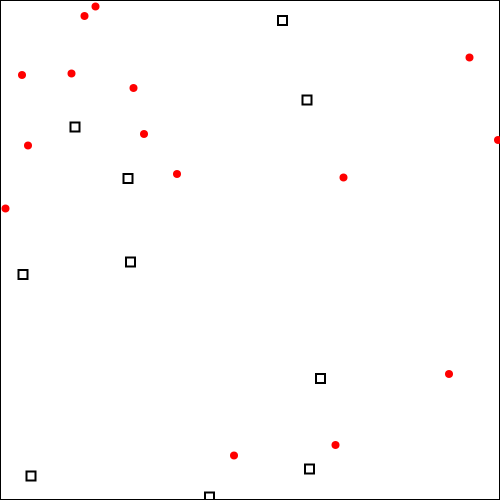
\includegraphics[width=5cm,height=5cm]{small_case_raw.png}}}
    \qquad \qquad \qquad
    \subfloat[Posible solución]{{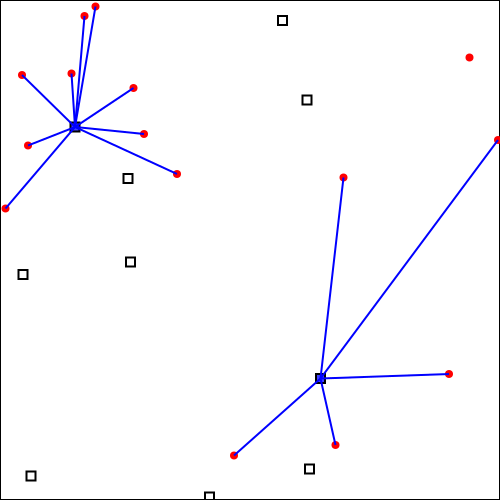
\includegraphics[width=5cm,height=5cm]{small_case_sol.png}}}
    \caption{A la izquierda, ejemplo de un problema, puntos rojos son ubicaciones de clientes, cuadrados son posibles ubicaciones de instalaciones.\\ A la derecha una posible solución, cuadrados azules representan subconjunto elegido de ubicaciones de instalaciones, clientes son trabajados por la instalación más cercana o ninguna si todas están muy lejos (tal es el caso del cliente en la esquina superior derecha).}
    \label{fig:problem}
\end{figure}

Notando que la función objetivo puede expresarse de la siguiente manera:
\begin{align*}
    -\sum_{j=1}^{|Z|} \gamma X_{j} + \sum_{i=1}^{|C|} w_i \sum_{j=1}^{|Z|} Y_{ij} (\alpha - \beta d_{ij})
\end{align*}
Se puede identificar un radio crítico $RC = \frac{\alpha}{\beta d_{ij}}$ pasado el cual no es conveniente suplir la demanda de un cliente. De la misma manera, puesto que la única variable controlable es $d_{ij}$, convendrá que la demanda de cliente sea suplida por la instalación colocada más cercana, a menos que esta se encuentre a una distancia mayor que el radio crítico.

Esta observación permite expresar una solución al problema ya no como el conjunto de varibles de decisión $X_{j}$ y $Y_{ij}$, sino como un subconjunto $S$ de $Z$, buscando maximiziar el valor de la siguiente función objetivo $\Phi : \mathcal{P}(Z) \rightarrow \mathbb{R}$:

\begin{equation}
\Phi(S) = -\gamma \cdot |S| + \sum_{i=1}^{|C|} \max \left\{ 0 , \max_{z \in S} ( \alpha \cdot w_i - \beta \cdot w_i \cdot d(c_i,z)) \right\}
\end{equation}

Una solución $S$ se traduce a una solución para el modelo de programación lineal, asumiendo por simplicidad y sin pérdida de generalidad que las distancias $d_{ij}$ son diferentes, de la siguiente manera:

\begin{align*}
    X_{j} &= \begin{cases}
        1 &\quad z_j \in S \\
        0 &\quad z_j \notin S
    \end{cases}\\
    Y_{ij} &= \begin{cases}
        1 &\quad (d_{ij} \leq RC) \wedge (d_{ij} \leq d_{ik} \quad \forall k : z_k \in S)
        \\
        0 &\quad e.o.c.
    \end{cases}
\end{align*}

Siendo las soluciones generadas de esta manera siempre igual o mejores que sus contrapartes con distintos valores $Y_{ij}$, se reduce el espacio de búsqueda, a uno con soluciones descritas completamente por un subconjunto de instalaciones elegido.

\section{Algoritmo}



\section{Reducción}

\section{Disimilitud}

\bibliographystyle{amsplain}
\bibliography{main}{}

\end{document}
